\section{Crowd Manager Message-Policy Selection}\label{sec:manager-selection}

A separate engine 1.4.0 experiment compared four message policies on 100 fresh audiences each (seeds 8001--8100). The six posts, activation and compliance draws, audience and physical parameters, and final-forty rule were identical across policies. No added LEDs or barriers were used. Only manager messages differed. Candidate configurations and selection criteria were recorded before completion of the experiment; no parameter was fitted to the results.

\begin{table}[htbp]\centering\small

\begin{tabularx}{\linewidth}{Xrrrr}\toprule

Policy & Complete & Mean (s) & 95\% interval (s) & $\leq180$ s\\\midrule

Nearest-time lower floor; original balcony exits & 100/100 & 178.7 & 176.6--180.9 & 55/100\\

Nearest-time from all six managers & 100/100 & 162.4 & 159.7--165.0 & 92/100\\

Fixed coordinated destinations & 100/100 & 177.2 & 175.1--179.3 & 68/100\\

Nearest-time lower floor; foyer from balcony & 100/100 & 163.3 & 160.7--165.9 & 91/100\\

\bottomrule\end{tabularx}

\caption{Fixed-policy comparison. Mean intervals quantify Monte Carlo sampling uncertainty, not physical or behavioural uncertainty.}\end{table}

\begin{figure}[htbp]\centering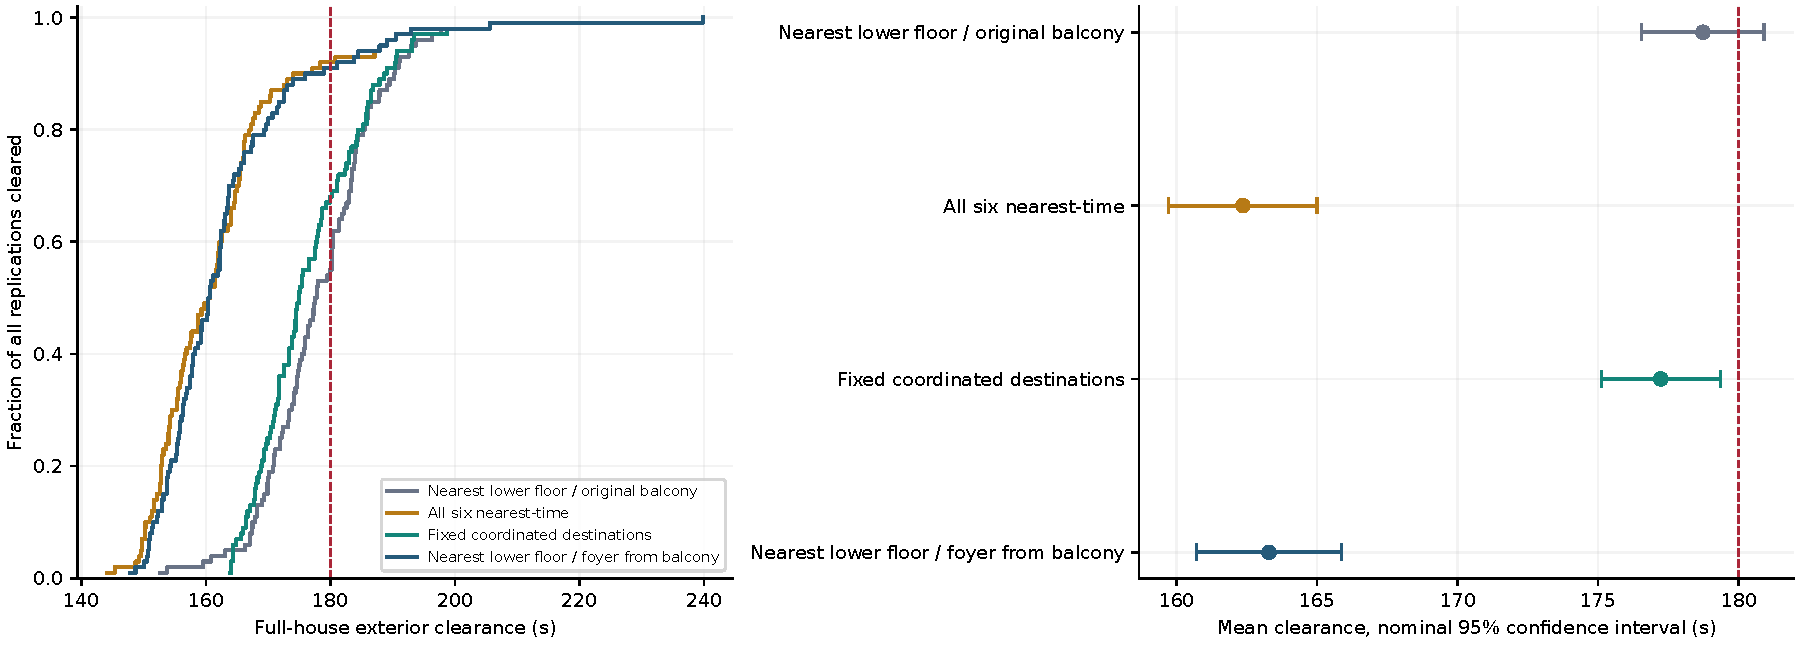
\includegraphics[width=\linewidth]{figures/manager-policy-comparison.pdf}

\caption{Empirical clearance distributions and nominal mean intervals for four manager policies. Dashed lines mark 180 seconds.}\end{figure}

The selected candidate is \textbf{Nearest-time from all six managers}. Lowest observed unconditional mean among fully completed policies.

The selected mean's simultaneous 95\% interval, adjusted over the four candidate means, is 158.98 to 165.74 s. This accounts for inspecting several means, but not physical or parameter uncertainty.

Relative to the requested lower-floor nearest-time policy with the original balcony exits, the selected policy's paired mean change is -16.37 s. Its simultaneous 95\% interval is -19.08 to -13.66 s.

\begin{table}[htbp]\centering\small

\begin{tabularx}{\linewidth}{llX}\toprule

Manager & Post & Public instruction\\\midrule

CM1 & \texttt{m1} & Nearest known feasible exit by estimated travel time\\

CM2 & \texttt{m4} & Nearest known feasible exit by estimated travel time\\

CM3 & \texttt{m8} & Nearest known feasible exit by estimated travel time\\

CM4 & \texttt{m11} & Nearest known feasible exit by estimated travel time\\

CM5 & \texttt{b4} & Nearest known feasible exit by estimated travel time\\

CM6 & \texttt{b8} & Nearest known feasible exit by estimated travel time\\

\bottomrule\end{tabularx}

\caption{Selected simulated messages. Posts are graph junctions, not approved standing positions.}\end{table}

The paired comparisons use Student-t intervals with Bonferroni simultaneous 95\% coverage across the six candidate contrasts. Selection uses the same sample, so it is not independent confirmation or a claim of global optimality. Unfinished runs remain in the success denominator and prevent an unconditional mean.

For implementation in the hall, fixed destination messages must map to clear local directions, with balcony foyer guidance using the appropriate rear stairs. Staff must remain clear of door swings and crowd movement, and speech and existing signs must agree. A generic nearest-time instruction assumes listeners can estimate route time from known exits and visible queues; this comprehension is not validated. The physical-placement limits in Section~\ref{sec:practical-review} remain applicable. These results do not authorize changing the venue emergency plan.


Nearest-time guidance keeps a single public instruction. Listeners evaluate known feasible routes using their current position and visible queues; managers do not periodically switch public destinations in response to congestion. The foyer-directed balcony variant is statistically close to the all-nearest variant; the adjusted interval for their paired difference includes zero. A selected sample minimum is not a proven unique optimum.

All 400 archives passed hash and crossing-count audits, with exact full-result replay of the first seed of each policy. All 741 final commitments were checked for connected routes and absence of later updates. The selected arm had 22 final commitments, including 12 exit changes, and 300/300 wheelchair-user observations reached the exterior and 300/300 reached street level within the horizon. The implementation passed 79 automated tests, 6 browser tests, TypeScript and the production build. The selected default reproduced its first-seed result completely after normalizing only the scenario title.
